% Copyright 2004 by Till Tantau <tantau@users.sourceforge.net>.
%
% In principle, this file can be redistributed and/or modified under
% the terms of the GNU Public License, version 2.
%
% However, this file is supposed to be a template to be modified
% for your own needs. For this reason, if you use this file as a
% template and not specifically distribute it as part of a another
% package/program, I grant the extra permission to freely copy and
% modify this file as you see fit and even to delete this copyright
% notice. 

\documentclass{beamer}

% There are many different themes available for Beamer. A comprehensive
% list with examples is given here:
% http://deic.uab.es/~iblanes/beamer_gallery/index_by_theme.html
% You can uncomment the themes below if you would like to use a different
% one:
%\usetheme{AnnArbor}
%\usetheme{Antibes}
%\usetheme{Bergen}
%\usetheme{Berkeley}
%\usetheme{Berlin}
%\usetheme{Boadilla}
%\usetheme{boxes}
%\usetheme{CambridgeUS}
%\usetheme{Copenhagen}
%\usetheme{Darmstadt}
%\usetheme{default}
%\usetheme{Frankfurt}
%\usetheme{Goettingen}
%\usetheme{Hannover}
%\usetheme{Ilmenau}
%\usetheme{JuanLesPins}
%\usetheme{Luebeck}
\usetheme{Madrid}
%\usetheme{Malmoe}
%\usetheme{Marburg}
%\usetheme{Montpellier}
%\usetheme{PaloAlto}
%\usetheme{Pittsburgh}
%\usetheme{Rochester}
%\usetheme{Singapore}
%\usetheme{Szeged}
%\usetheme{Warsaw}

\usepackage{kotex}
\usepackage{braket}
\usepackage{array}
\usepackage{calc}
\usepackage{datetime}


\usepackage{listings}


\title{Lecture 1.5 :git/LaTeX}

% A subtitle is optional and this may be deleted
\subtitle{Fastcampus Math Camp}

\author{신승우}
% - Give the names in the same order as the appear in the paper.
% - Use the \inst{?} command only if the authors have different
%   affiliation.

% \institute[Universities of Somewhere and Elsewhere] % (optional, but mostly needed)
% {
  % \inst{1}%
  % Department of Computer Science\\
  % University of Somewhere
  % \and
  % \inst{2}%
  % Department of Theoretical Philosophy\\
  % University of Elsewhere}
% - Use the \inst command only if there are several affiliations.
% - Keep it simple, no one is interested in your street address.

% - Either use conference name or its abbreviation.
% - Not really informative to the audience, more for people (including
%   yourself) who are reading the slides online

\subject{Theoretical Computer Science}

% This is only inserted into the PDF information catalog. Can be left
% out. 

% If you have a file called "university-logo-filename.xxx", where xxx
% is a graphic format that can be processed by latex or pdflatex,
% resp., then you can add a logo as follows:

% \pgfdeclareimage[height=0.5cm]{university-logo}{university-logo-filename}
% \logo{\pgfuseimage{university-logo}}

% Delete this, if you do not want the table of contents to pop up at
% the beginning of each subsection:


\AtBeginSection[]
{
  \begin{frame}<beamer>{Outline}
    \tableofcontents[currentsection,hideallsubsections]
  \end{frame}
}

% Let's get started
\begin{document}

\begin{frame}
  \titlepage
\end{frame}

\begin{frame}{Outline}
  \tableofcontents[hideallsubsections]
  % You might wish to add the option [pausesections]
\end{frame}

% Section and subsections will appear in the presentation overview
% and table of contents.

\section{Introduction to Git} 

\subsection{git 소개} 

\begin{frame}{Git 설치}

$\sum^{n}_{i=1}$
\begin{itemize} 
\item Windows : git-scm 설치 (http://git-scm.com/download/win)
\item Linux(Ubuntu) : sudo apt-get install git
\item Mac : git-scm 설치 (http://git-scm.com/download/mac)
\end{itemize}
\end{frame}

\begin{frame}{Git 이란?}
\begin{itemize}
\item 버전 관리 툴(VCS: Version Control System)
\item Made by 'The' Linus Benedict Torvalds
\end{itemize}
\end{frame}

\begin{frame}{Local VCS}
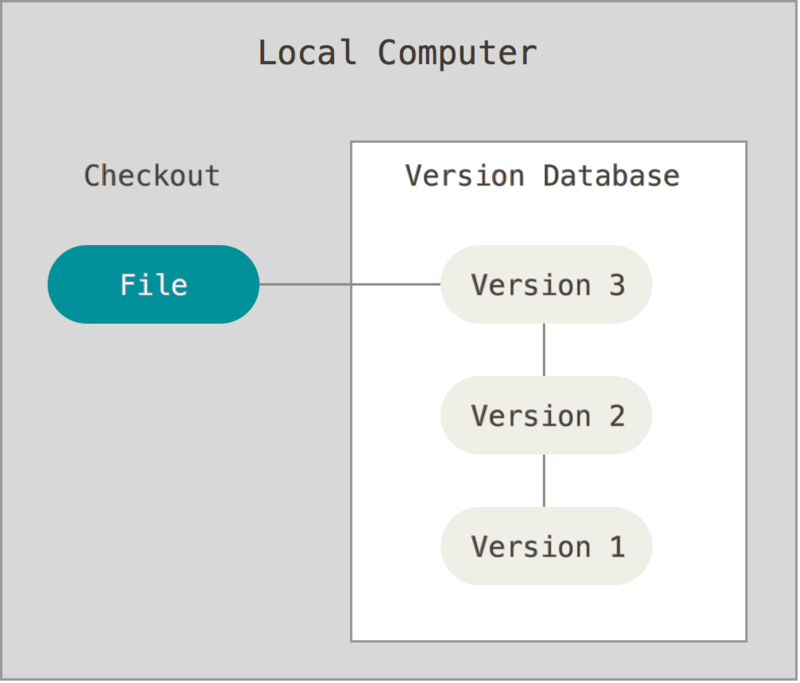
\includegraphics[height=5cm,keepaspectratio]{local}
\end{frame}

\begin{frame}{Centralized VCS}
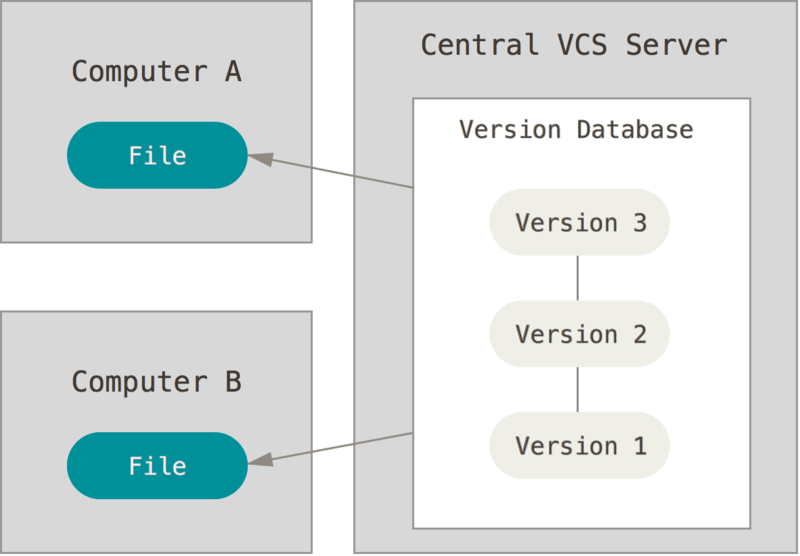
\includegraphics[height=5cm,keepaspectratio]{centralized}
\end{frame}

\begin{frame}{Distributed VCS}
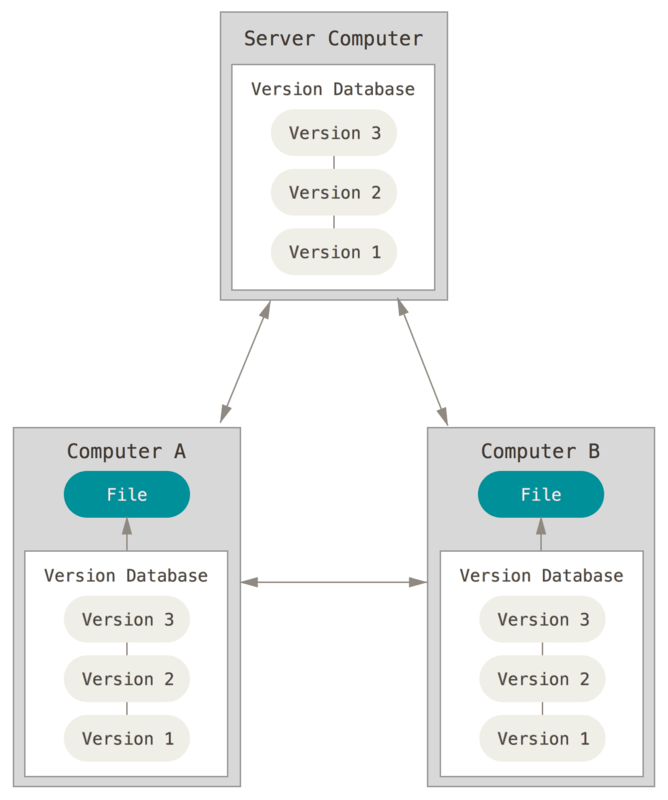
\includegraphics[height=5cm,keepaspectratio]{distributed}
\end{frame}





\begin{frame}{Git 환경설정}
\begin{itemize} 
\item 사용자 정보 설정 \\
 git config --global user.name "John Doe" \\
 git config --global user.email johndoe@example.com

\item 편집기 설정 

 git config --global core.editor emacs (emacs user) \\
 git config --global core.editor "path to editor exe"

\end{itemize}
\end{frame}


\subsection{git repo 관리하기}


\begin{frame}{Git 저장소 만들기}

\begin{itemize} 
\item git init : 새로 만들기 
\item git clone : 기존 저장소 복사 
\end{itemize}
\end{frame}

\begin{frame}{Git 안에서 파일의 life cycle 이해}
깃은 Snapshot을 저장하는데, 여기서 스냅샷을 '찍는' 행위를 커밋이라고 합니다. 
깃은 커밋 시마다 모든 파일의 복사, 압축본을 만들어 저장합니다. 
\end{frame}
\begin{frame}{Git 안에서 파일의 life cycle 이해}
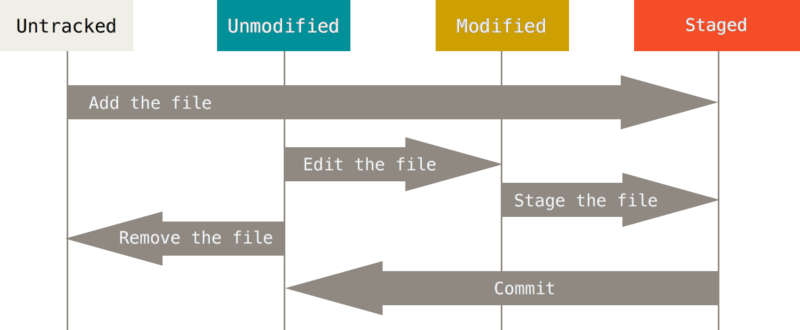
\includegraphics[height=5cm,keepaspectratio]{lifecycle}
\end{frame}

\begin{frame}{Git 안에서 파일의 life cycle 이해}
\begin{itemize} 
\item Tracked/Untracked : 추적 여부. git add로 추적 시작, git remove로 추적 종료
\item Tracked Files
\begin{itemize} 
\item Staged : commit 직전
\item Modified : commit 후 수정됨
\item Unmodified : commit 직후
\end{itemize}
\end{itemize}
\end{frame}


\begin{frame}{Git 안에서 파일의 life cycle 이해 : .gitignore}
특정 파일은 항상 무시하고 싶을 때, 매번 일일히 add를 할 수는 없다. 따라서 보통 git add . 으로 모든 파일을 add하게 되는 경우가 많은데, 이 때 원하지 않는 형식의 파일은 add하면 안 된다. 
\begin{itemize} 
\item 확장자 : *.py 형식 
\item 무시하는 것에서 예외 : !test.py 
\item 현 디렉토리 파일만 무시 : /TODO
\item 특정 디렉토리 무시 : build/
\item 특정 디렉토리 아래의 특정 확장자 무시 : doc/**/*.py
\item 주석 : \# 
\end{itemize}
\end{frame}


\begin{frame}{Git에서 수정 후 커밋해보기}
일반적으로 다음의 과정을 따른다. 
\begin{itemize} 
\item git init/git clone으로 저장소 시작 
\item 파일 수정 
\item git add filename (혹은 git add .) 
\item git commit -m 'commit message' : 커밋 메세지 없이는 커밋되지 않으며, -m 플래그를 쓰지 않으면 자동으로 위에서 설정한 에디터가 켜집니다. 
\item git pull origin master : 협업자와 같이 remote에서 작업할 경우 
\item git push origin master : remote에서 작업할 경우
\end{itemize}
\end{frame}


\begin{frame}{Git 에서 전 상태로 되돌리기 : 커밋 수정하기}
git commit --amend \\
로 마지막 커밋을 수정한다. 커밋 메세지를 바꾸거나, 파일을 빠트렸거나 할 때 사용한다. 이 때, 새로운 커밋은 마지막 커밋을 덮어쓰게 된다. 예를 들어, 다음의 명령어는 하나의 커밋만을 만든다. 

git commit -m 'hello!' \\
git add forgottenfile \\
git commit -amend \\
\end{frame}




\begin{frame}{remote 저장소와 Github}
git remote로 remote 저장소를 관리한다. 

\begin{itemize} 
\item git remote : 리모트 저장소의 목록을 보여준다. -v를 쓸 경우, url까지 보여준다. 
\item git remote add : 리모트 저장소를 추가한다. \\
git remote add origin 'https://github.com/yourid/repourl'
\end{itemize}

\end{frame}

\begin{frame}{Remote에 push하기}
git push remote-name branch-name\\
으로 리모트 저장소로 나의 작업을 push할 수 있다. 다만, 여기서 두 가지 조건이 필요한데 
\begin{itemize} 
\item 쓰기 권한이 있어야 함
\item 다른 사람의 작업본을 로컬에서 최신 버젼으로 업데이트했어야 함
\end{itemize}
\end{frame}

\subsection{git branch} 

\begin{frame}{More on Git Structure - commit internal} 
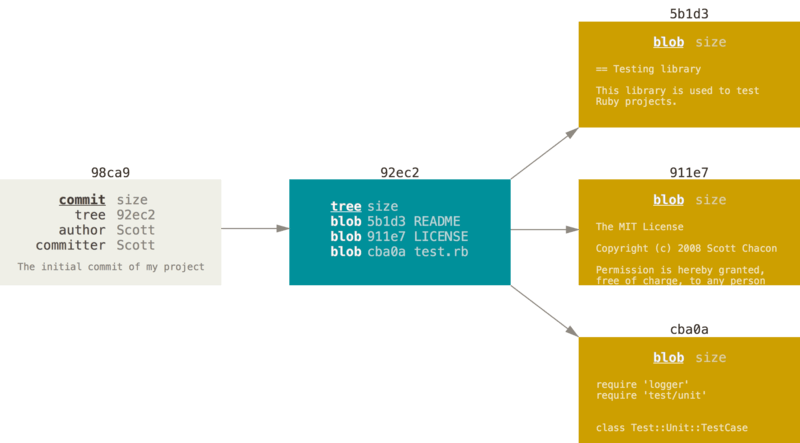
\includegraphics[height=5cm,keepaspectratio]{commit-and-tree}
\end{frame}

\begin{frame}{More on Git Structure - commits} 
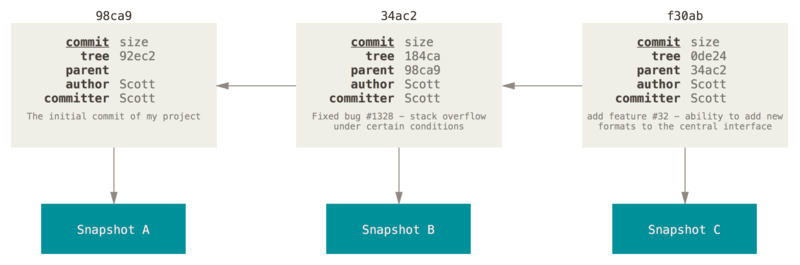
\includegraphics[height=3.5cm,keepaspectratio]{commits-and-parents}
\end{frame}

\begin{frame}{More on Git Structure - branch} 
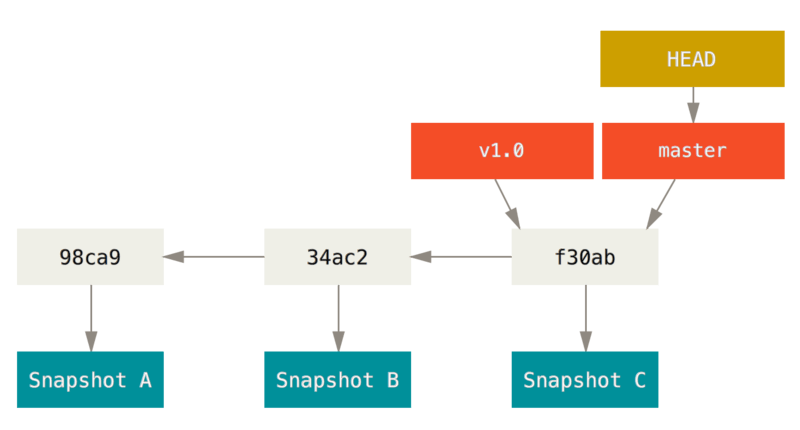
\includegraphics[height=5cm,keepaspectratio]{branch-and-history}
\end{frame}

\begin{frame}{More on Git Structure - new branch} 
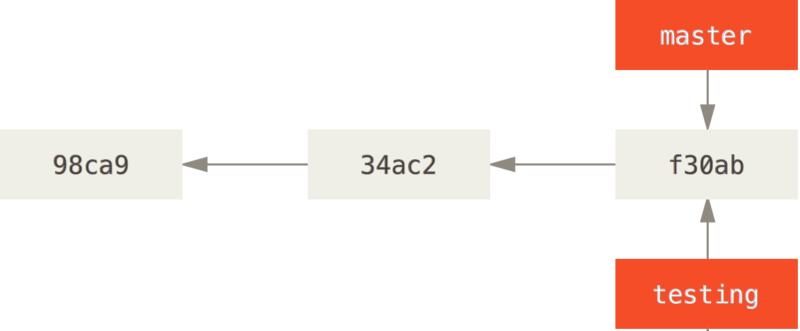
\includegraphics[height=5cm,keepaspectratio]{two-branches}
git branch testing으로 새 브랜치를 생성
\end{frame}


\begin{frame}{More on Git Structure - HEAD} 
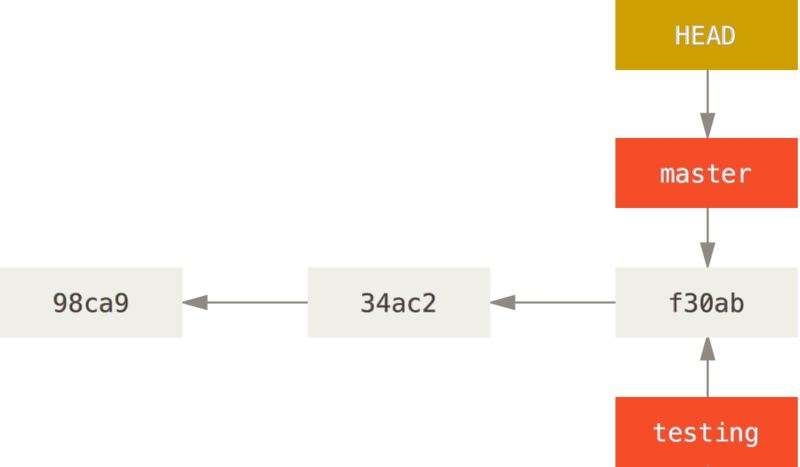
\includegraphics[height=5cm,keepaspectratio]{head-to-master} \\
HEAD는 특수한 포인터로, 지금 작업 중인 branch를 가리킴. 
\end{frame}


\begin{frame}{More on Git Structure - move HEAD} 
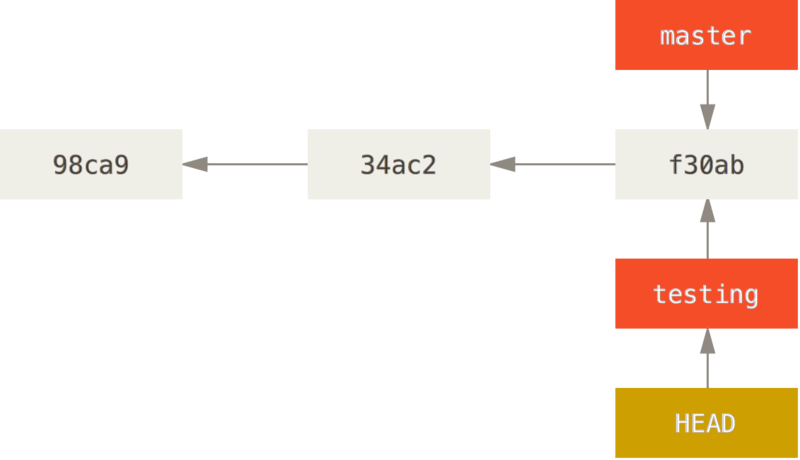
\includegraphics[height=5cm,keepaspectratio]{head-to-testing} \\
git checkout 명령어로 작업 중인 branch를 바꿀 수 있음. 이 때 HEAD가 이동함. 
\end{frame}


\begin{frame}{More on Git Structure - new commit} 

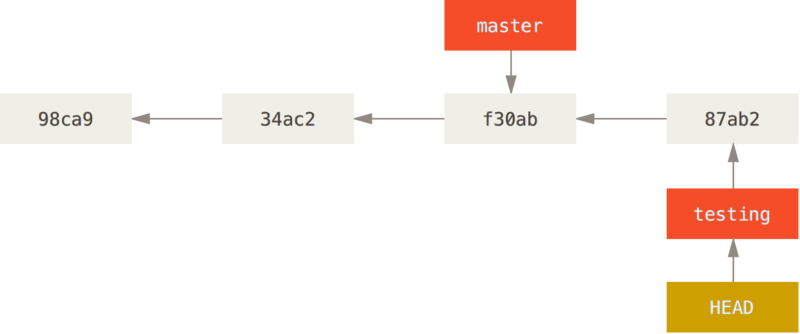
\includegraphics[height=5cm,keepaspectratio]{advance-testing}
이후, 수정하고 커밋을 해 보면 위와 같다.
\end{frame}


\begin{frame}{More on Git Structure - new branch} 

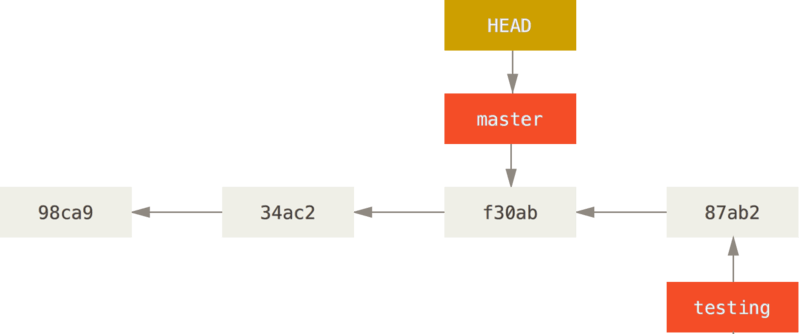
\includegraphics[height=5cm,keepaspectratio]{checkout-master}
git branch testing으로 새 브랜치를 생성하면 위와 같이 됨. 
\end{frame}


\begin{frame}{More on Git Structure} 
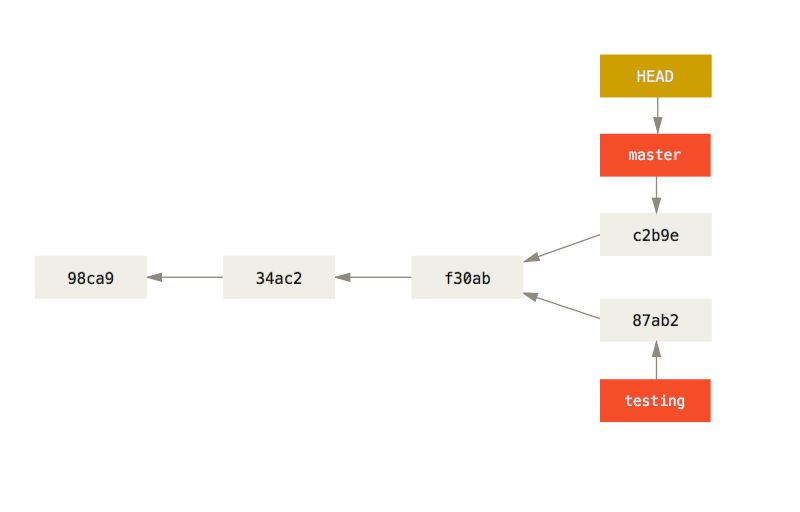
\includegraphics[height=5cm,keepaspectratio]{advance-master} \\
master branch를 수정하여 커밋하였으므로 그림처럼 branch가 나눠지게 됨. 
\end{frame}


\begin{frame}{Git Branch를 이용한 문제 해결 : Hotfix Issue}
웹사이트 개발 프로젝트를 진행하는 중, 새로운 기능을 넣고 있습니다. 이 때 급하게 고쳐야 하는 hotfix가 있다고 합시다. 기존 진행중이던 기능 개발을 최대한 영향 주지 않으면서 일단 hotfix를 진행하고자 합니다. 이 때 어떤 식으로 버젼관리를 해야 할까요?  
\end{frame}

\begin{frame}{Git Branch를 이용한 문제 해결 : Hotfix Issue} 

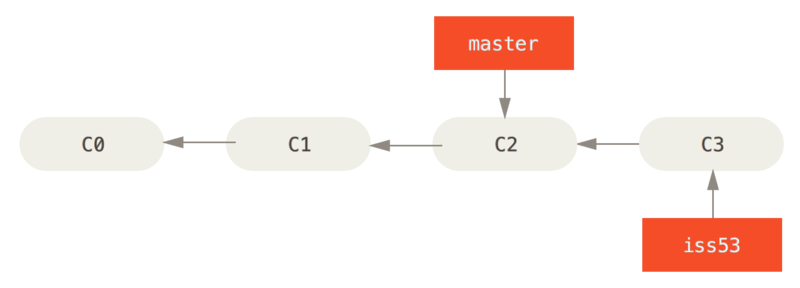
\includegraphics[height=3.5cm,keepaspectratio]{develop}  \\
기능 개발 부분이 iss53 브랜치라고 하고, 지금 진행중인 상태를 나타내면 위와 같음. 
\end{frame}



\begin{frame}{Git Branch를 이용한 문제 해결 : Hotfix Issue} 

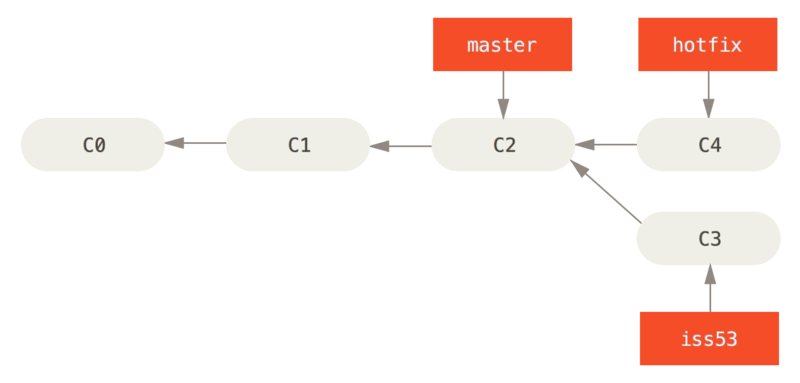
\includegraphics[height=5cm,keepaspectratio]{basic-branching-4}  \\
이 때, hotfix를 위해서 새로운 branch hotfix를 하나 만듬. //
git checkout -b hotfix
\end{frame}



\begin{frame}{Git Branch를 이용한 문제 해결 : Hotfix Issue} 

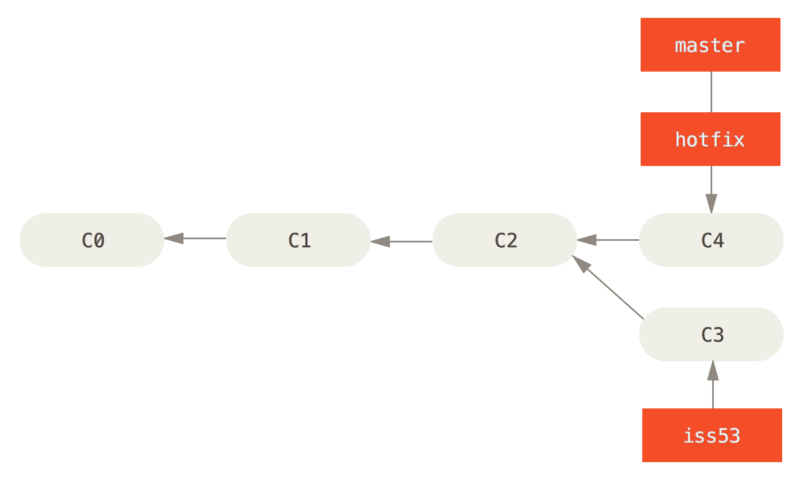
\includegraphics[height=5cm,keepaspectratio]{basic-branching-5}  \\
이후 hotfix가 진행되어서, 문제가 해결되면 master를 hotfix와 merge    
git checkout master\\ 
git merge hotfix \\

이런 형태의 merging을 fast-forward라고 합니다. (직계 조상인 경우)
\end{frame}

\begin{frame}{Git Branch를 이용한 문제 해결 : Hotfix Issue} 

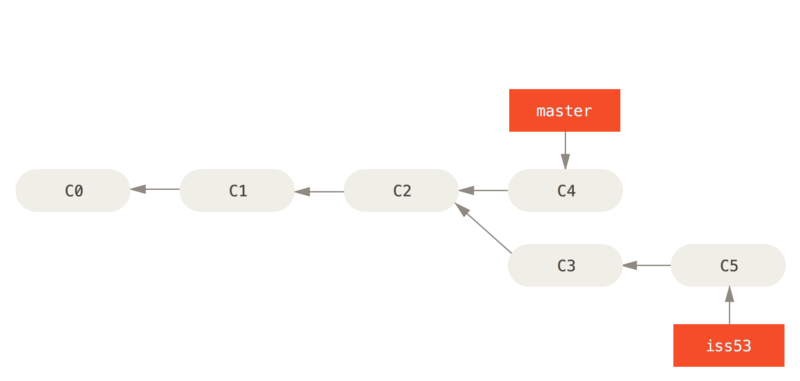
\includegraphics[height=5cm,keepaspectratio]{basic-branching-6} \\
이 때, 동시에 iss53은 독립적으로 진행 가능
\end{frame}

\begin{frame}{Git Branch를 이용한 문제 해결 : Hotfix Issue} 

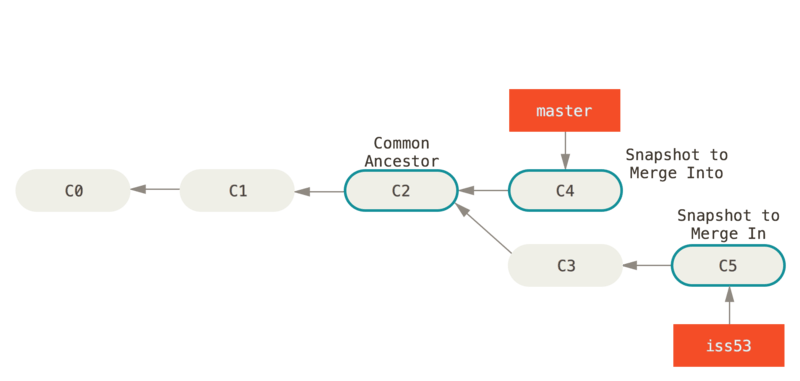
\includegraphics[height=5cm,keepaspectratio]{basic-merging-1}  \\
이제 iss53이 잘 개발이 끝났으므로, master branch와 merge 시도. 이 경우, 공동 조상이 없으므로 가장 가까운 common ancestor를 찾아 merge를 시도한다. \\
git merge iss53
\end{frame}

\begin{frame}{Git Branch를 이용한 문제 해결 : Hotfix Issue} 
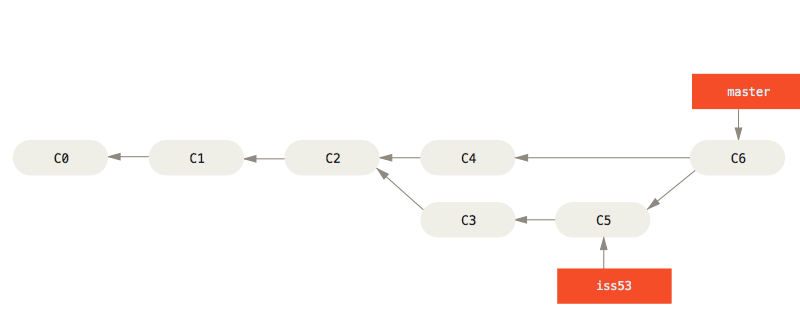
\includegraphics[height=3.5cm,keepaspectratio]{basic-merging-2}  \\
해결이 완료되면 위와 같이 된다. 
\end{frame}

\begin{frame}{Merge Conflict} 
만약, 두 커밋에서 같은 파일의 같은 부분을 다르게 수정했다면 문제가 생긴다. 이런 경우를 merge conflict라고 한다. mergetool을 쓰거나, 수동으로 merge할 수 있다. 
\end{frame}

\begin{frame}{More on Branching : Remote Branch}
이때까지는 local에서 혼자 작업하는 경우를 고려하였다. 이제, remote에서 협업할 때 어떤 식으로 branching이 사용되는지 살펴보겠다. 
\end{frame}


\begin{frame}{More on Branching : Remote Branch}
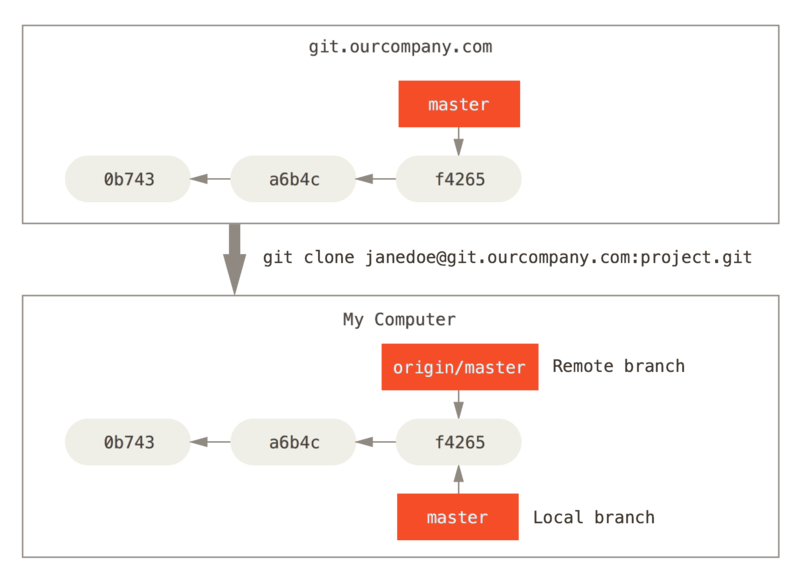
\includegraphics[height=5cm,keepaspectratio]{remote-branches-1} \\
git clone을 사용하여 remote branch를 복사해온다. 
\end{frame}

\begin{frame}{More on Branching : Remote Branch}
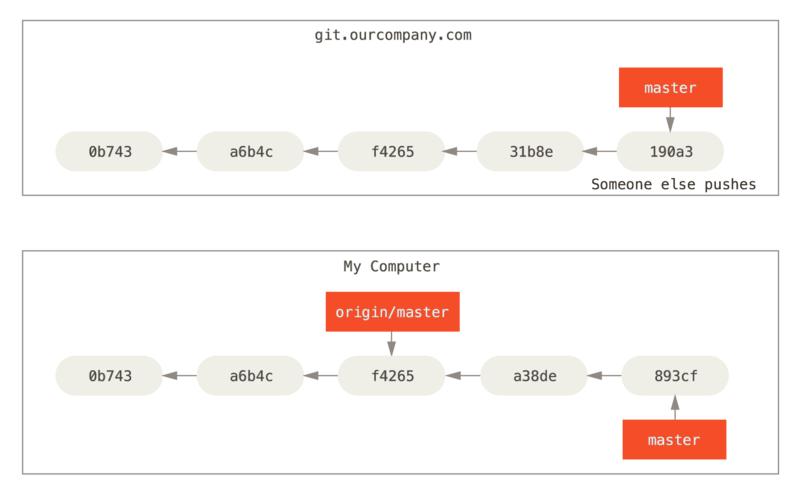
\includegraphics[height=5cm,keepaspectratio]{remote-branches-2} \\
그 후, remote와 local에서 독립적으로 작업이 진행되었다고 하자.
\end{frame}


\begin{frame}{More on Branching : Remote Branch}
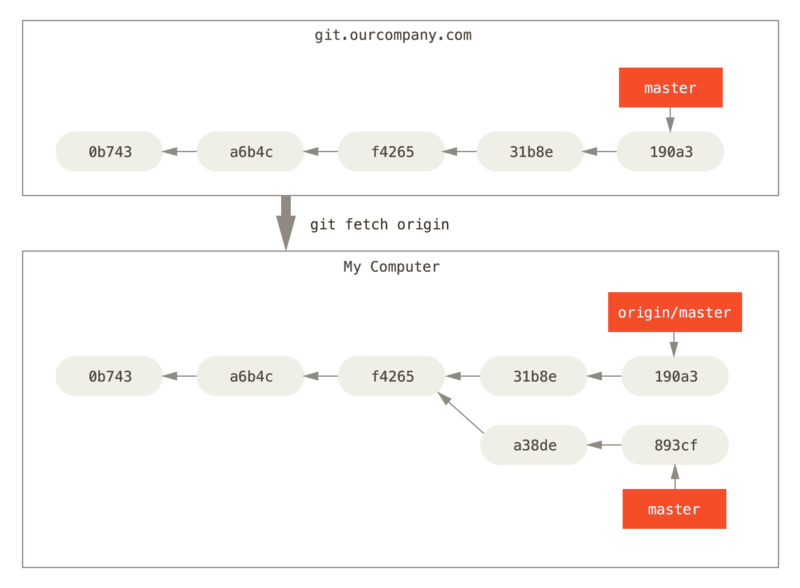
\includegraphics[height=5cm,keepaspectratio]{remote-branches-3} \\ 
이 때, fetch나 pull을 이용하여 작업된 부분을 받아올 수 있다.
\end{frame}

 
\begin{frame}{More on Branching : fetch vs pull}
fetch와 pull은 둘 다 리모트 서버에서 데이터를 받아오는 방법이다. 하지만, 그 후 자동으로 merge를 수행하는지에 대한 차이가 있다. 즉, \\
git fetch origin master \\
git merge origin/master \\
과 \\
git pull origin master \\
은 같은 작업이다. 일반적으로는 전자가 권장된다. 
\end{frame}


\section{Introduction to LaTeX} 

\subsection{LaTeX 소개} 


\begin{frame}{LaTeX 설치}
\begin{itemize}
\item 로컬 : https://www.latex-project.org/get/ 에서 해당되는 OS로 설치 
\item 웹 
\begin{itemize}
\item overleaf : https://www.overleaf.com/
\item sharelatex : https://www.sharelatex.com/project
\end{itemize}
\end{itemize}
\end{frame}

\begin{frame}{LaTeX}
\begin{itemize}
\item 조판(Typesetting) 시스템: 스타일과 내용의 분리!     
\item Made by 'The' Knuth 
\end{itemize}
\end{frame}

\subsection{LaTeX 문법} 


\begin{frame}{LaTeX 문법}
\begin{itemize} 
\item html과 매우 비슷함 
\item \textbackslash 으로 명령어 시작 : \textbackslash command\{argument\}
\item \textbackslash begin\{environment\}로 특정 환경 시작. ex)lstlisting, equation 등
\item chapter, section, subsection으로 문서 구성 
\end{itemize}
\end{frame}

\begin{frame}{LaTeX - Using the Package} 
\textbackslash usepackage\{packagename\}으로 사용. 대표적인 패키지들은
\begin{itemize} 
\item kotex : 한국어 사용
\item lstlisting : 소스 코드 임베딩 
\item graphicsx : 그래픽 관련. 그림 그리거나 등등 
\item hyperref : 하이퍼링크용 
\item lipsum : 템플릿용 dummy text 
\end{itemize}
\end{frame} 




\begin{frame}{LaTeX - Using the Template} 
템플릿을 이용하는 법은 상황 따라 다른데, 
\begin{itemize} 
\item .cls파일 제공 : documentclass
\item .sty파일 제공 : usepackage
\end{itemize}
\end{frame} 

\begin{frame}{LaTeX - Equation} 
LaTeX에서는 강력한 수식 입력 툴을 제공하는데, 기본적으로는 hwp 수식입력기와 비슷하다. 
\begin{itemize} 
\item \$\$ 환경 
\item equation 환경 
\end{itemize}
\end{frame} 



\begin{frame}{LaTeX : Look at the code} 
\begin{itemize} 
\item 논문 조판 
\item 교재 조판 
\item ppt 조판 
\end{itemize}
\end{frame} 




\subsection{LaTeX 팁} 

\begin{frame}{LaTeX 팁}
\begin{itemize}
\item detexify : \href{http://detexify.kirelabs.org/}{http://detexify.kirelabs.org/}
\item latex table generator : \href{https://www.tablesgenerator.com/}{https://www.tablesgenerator.com/}
\end{itemize}
\end{frame}


\end{document}


